\Titular*%
{Coñecendo a Ana Ulla Miguel}%
{Gemma Ruíz Lavandeira}%
{entrevistas}%
{Conversa de tal coa astrofísica Ana Ulla Miguel.}%

\begin{refsection}
\begin{multicols}{2}

\subsection*{Biografía}
Ana Ulla Miguel comezou a licenciatura en Ciencias Físicas na Universidade de
Santiago de Compostela, para logo especializarse en astrofísica na Universidad
de La Laguna, lugar onde obtería o seu título de doutora en 1993. Entre 1988 e
1995, ocupou diversos postos de investigación e docencia na Universidade de
Tromsø (Noruega), o Laboratorio de Astrofísica Espacial e Física Fundamental
(Madrid), a \textit{Axencia Espacial Europea} (ESA) ou o Instituto Niels Bohr
(Copenhague). Posteriormente, foi contratada posdoutoral no Instituto de
Astrofísica de Canarias (IAC), traballando no proxecto ``\textit{Infrared
Space Observatory}'' (ISO) da ESA.

\begin{center}
    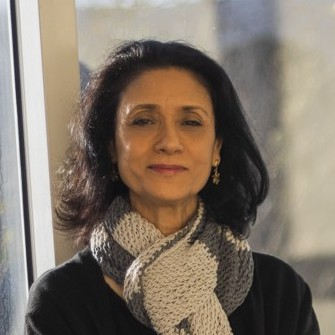
\includegraphics[width=0.85\linewidth]{revistas/002/imaxes/PHOTO-2025-04-30-18-18-48.jpg}
    \captionof{figure}{Ana Ulla Miguel.}
\end{center}

Dende 1997 é docente do Departamento de Física Aplicada da Universidade de
Vigo, sendo a investigadora principal do Grupo AS1 de Astronomía e Astrofísica
da UVIGO dende a súa creación no ano 2005 ata outubro de 2017. Dende 2022 é
catedrática de astronomía e astrofísica do mesmo departamento e investigadora
do grupo GEOMA (\textit{Xeoloxía Mariña e Ambiental}) integrado no CIM
(\textit{Centro de Investigación Mariña}) da UVIGO. Os seus intereses de
investigación inclúen, entre outros temas, a evolución estelar en fases
avanzadas, os exoplanetas ou a astrobioloxía. Forma parte do grupo galego da
misión Gaia, da ESA, xunto con outros compañeiros da Universidade da Coruña
(UDC) e a Universidade de Cantabria (UNICAN).

\subsection*{Entrevista}%Preguntas}

\paragraph{Gemma:} En primeiro lugar, Ana, moitas grazas por participar na nosa
revista e acceder a contestar unhas preguntas para coñecer máis sobre ti e
sobre o teu traballo. É un grande orgullo poder contar co teu testemuño. Para
comezar, poderías contarnos como xurdiu o teu interese por estudar Física e
posteriormente Astrofísica?

\paragraph{Ana:} Grazas a vós por convidarme para esta entrevista e parabéns pola
iniciativa da vosa revista.

Dende a adolescencia souben que quería entender o mundo e o universo, ou
intentalo polo menos. Buscando información (e daquela non había nin Internet,
nin móbiles nin ordenadores) descubrín que, para formarme como astrofísica, o
camiño natural era estudar física primeiro e especializarme en astrofísica
despois. Ao final, isto pasaba por escoller o bacharelato de ciencias en Vigo,
física en Santiago e astrofísica en La Laguna. E así fixen.

\paragraph{G:} Ademais formas parte do equipo galego que participa na misión Gaia
da Axencia Espacial Europea. Non parece fácil, pero cal é o camiño para poder
traballar e colaborar coa ESA? Hai facilidades para estudantes de todos os
lugares para poder traballar nun futuro aí?

\paragraph{A:} Os meus primeiros contactos coa ESA foron hai moitos anos, como
observadora cun dos seus históricos satélites, o IUE (\textit{International
Ultraviolet Explorer}), en Madrid, sendo aínda estudante de doutoramento.
Despois, traballei por un período breve no seu centro de ESRIN (\textit{ESA
Centre for Earth Observation}), en Italia, logo traballei co equipo do satélite
ISO no IAC en Tenerife a cargo de Francisco Garzón e, dende aproximadamente
2007, colaboro co grupo de Minia Manteiga, da UDC, no satélite Gaia, que é unha
das grandes misóns da ESA para este século.

Hai moitas posibilidades de colaborar coa ESA, en múltiples formas, e hai
moitas oportunidades para estudantes, especialmente de física ou enxeñarías.
Por exemplo, cunha busca online bastante simple, atopas directamente na web da
ESA  “\textit{Current opportunities for university students}”. Eu animo a todo
o mundo que o queira intentar que busque estas oportunidades, porque na ESA hai
proxectos interesantísimos e con enorme proxección de futuro.

\paragraph{G:} A misión Gaia ten como principal obxectivo mapear
tridimensionalmente a Vía Láctea. No proceso, acádanse novos descubrimentos,
ata o punto de que a propia ESA a describe como a ``máquina de descubrimento
definitiva". Cal é para ti a maior satisfacción da misión Gaia? E a maior
dificultade que presentou ou aínda presenta este proxecto?

\paragraph{A:} O noso grupo intégrase no que se coñeece como DPAC (\textit{Data
Processing and Analysis Consortium}), unha colaboración paneuropea con máis de
catrocentos cincuenta investigadores/as e tecnólogos/as de máis de vinte
países. O obxectivo principal é a produción do catálogo final de datos de Gaia,
cunha enorme complexidade de procesamento, validación e distribución, pero que
quedará realmente como un legado científico de grande valor, para a humanidade.

Para min, só o feito de poder participar nunha colaboración internacional como
esta xa me resulta moi satisfactorio, especialmente traballando con colegas da
UDC e da UNICAN. E, ao mesmo tempo, considero que a complexidade de
funcionamento deste proxecto imparte moitas leccións importantes sobre a
colaboración científica e humana en xeral, que ben poderiamos extrapolar a
outros campos do coñecemento ou do traballo. Agora que o satélite, despois de
máis de once anos, xa non pode adquirir máis datos científicos, traballar cara
a elaboración do catálogo final é o reto definitivo, e bastante complexo, que
nos queda por abordar.

\begin{center}
    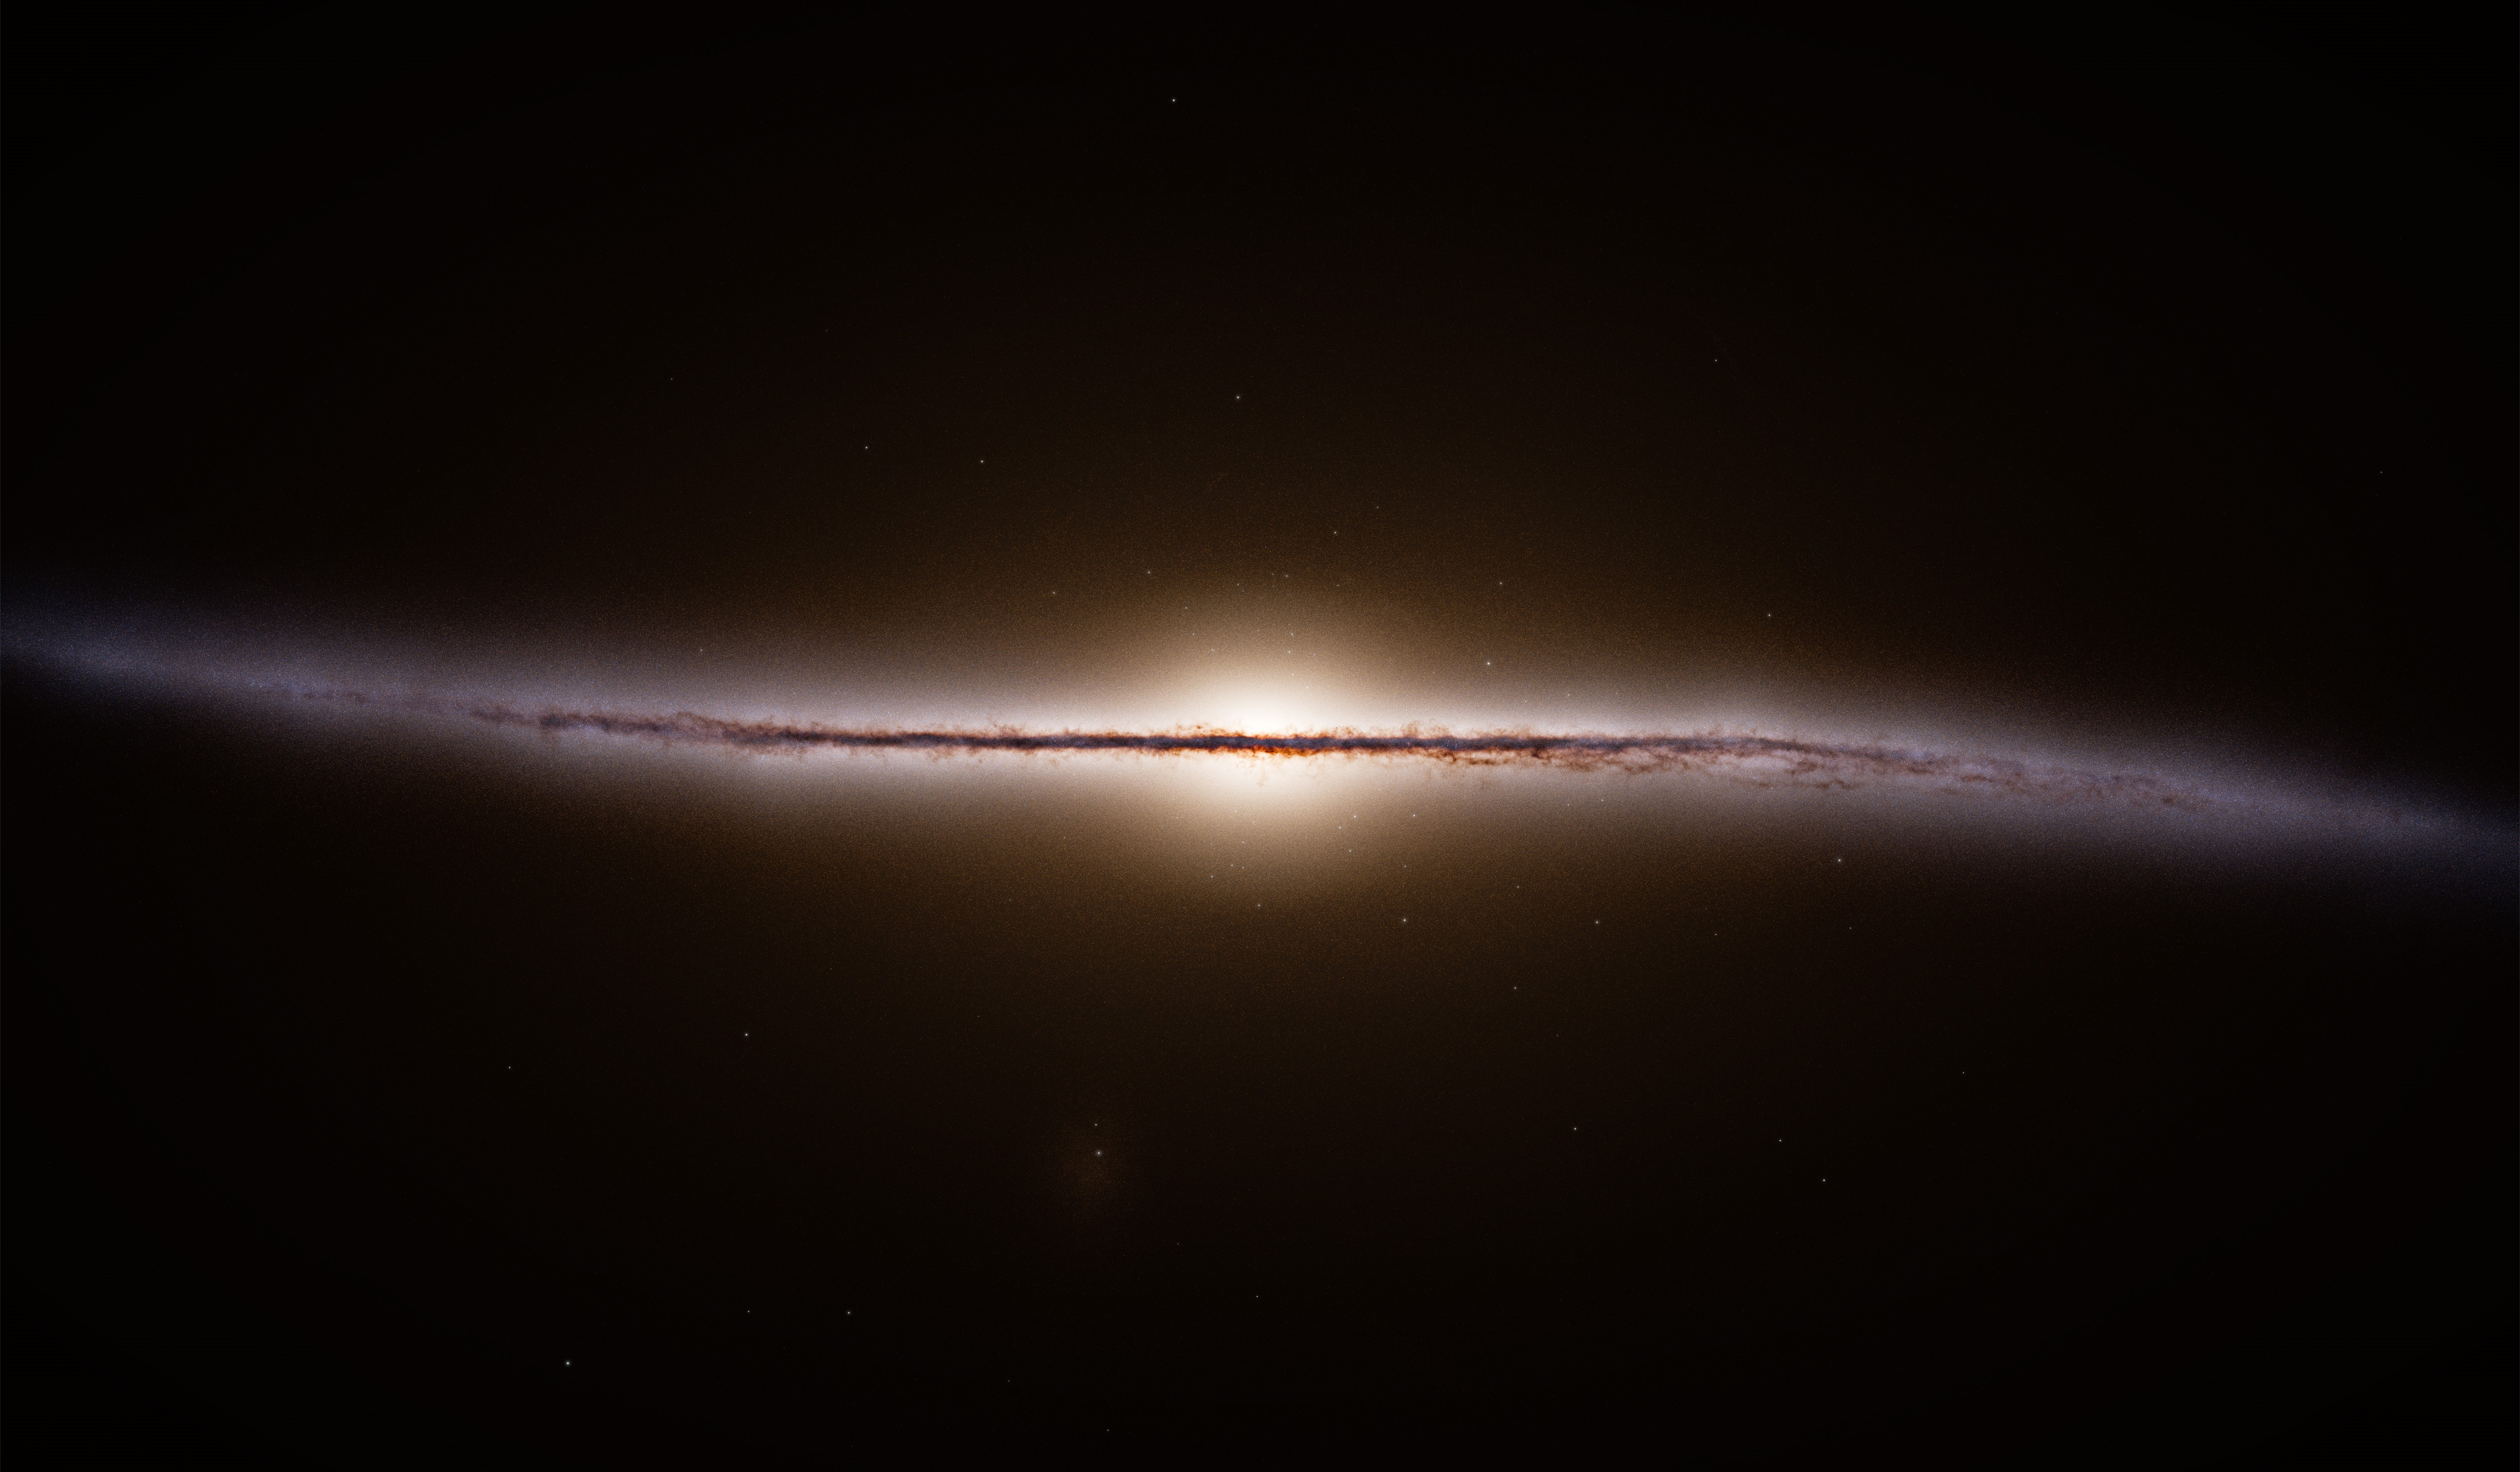
\includegraphics[width=1\linewidth]{revistas/002/imaxes/vialactea.jpg}
    \captionof{figure}{Foto da Vía Láctea polo proxecto Gaia. Image Credit: ESA/Gaia/DPAC, por Stefan Payne-Wardenaar}
\end{center}

\paragraph{G:} O ano pasado foi bastante notoria a noticia de que descubrirades un
buraco negro bastante masivo na Vía Láctea.Ti participaras neste achado, cal é
o proceso ata obter os resultados? Sodes partícipes durante todo o proceso do
que se está a descubrir ou analizades os datos a cegas? Que información aportan
estes buracos negros para comprender mellor a galaxia?

\paragraph{A:} Todos os datos de Gaia procésanse masivamente e de xeito
sistemático para depurar resultados espurios e logo facer clasificacións por
categorías, etc. E de cando en vez hai sorpresas ou verdadeiros descubrimentos,
coma no caso deste buraco negro estelar que, de momento, é o máis masivo na
galaxia. No procesado global dos datos traballamos todo DPAC en grupos de
traballo e, dentro destes grupos, un equipo particular foi o que fixo a análise
detallada do descubrimento.

Este tipo de buracos negros (BNs) correspóndense cos estadíos evolutivos finais
das estrelas máis masivas, que morren violentamente en forma de supernovas. E
as estrelas, coa súa evolución, en xeral moldean a evolución química das
galaxias que as conteñen; iso como mínimo. En particular, os BNs son
laboratorios formidables para avanzar no estudo da relatividade xeral e para
poñer a proba o alcance das leis da física. Tamén, para estudar as súas
posibles diferenzas de comportamento cos buracos negros supermasivos dos
interiores galácticos, e para progresar no que se coñece como astronomía
multimensaxeiro que combina información electromagnética e de ondas
gravitacionais. Digamos que son obxectos extremos e exóticos de grande
utilidade e bastante versátil en investigación.

\paragraph{G:} Gustaríame preguntar polas colaboracións internacionais. En
proxectos de tan grande escala a participación de grupos de traballo de
diversos países entendo que é imprescindible: é fácil unir a xente de varios
lugares para traballar en equipo ou é un traballo máis independente? Consideras
que hai unha búsqueda de coñecemento e respostas en todo o mundo ou hai países
máis proclives e outros que non prestan tanta colaboración?

\paragraph{A:} Efectivamente, a colaboración internacional, pero a todas as
escalas en realidade, é imprescindible para a consecución de obxectivos. A
astrofísica leva a colaboración científica implícita no ADN, diría eu. Para min
foi case unha das primeiras ferramentas de traballo que aprendín xa na etapa da
especialización, antes do doutoramento.

E canto máis ambiciosos os obxectivos (exploración espacial, vida
exoplanetaria, expansión acelerada do universo...) maiores e máis amplas
colaboracións que tecemos. Da miña experiencia, e ate onde eu sei, en
astrofísica colaboramos de todos os xeitos que se precise e por todas as partes
do mundo, unha vez definido o proxecto e os obxectivos que corresponda. Creo
que só así se pode entender o enorme avance desta disciplina e, paralelamente,
do noso coñecemento do universo dende hai pouco máis dun século.

\paragraph{G:} Unha cuestión que se plantexa máis dalgunha estudiante é se a
ciencia é un espazo igualitario, se a búsqueda do coñecemento está exenta de
estereotipos e se en xeral é un espazo afable. Queda camiño por percorrer ou a
situación é positiva ao respecto?

\paragraph{A:} Eu coñezo moitas colegas con recoñecidísimas traxectorias
profesionais, desenvoltas no espazo científico que hai. Ese espazo e tan
igualitario coma o espazo social e laboral no que se inxira. En España hai
arredor dun 30\% de astrofísicas, pero esta porcentaxe é menor nalgúns paises.
E nas universidades españolas hai aproximadamente un 25\% de catedráticas e un
75\% de catedráticos. Creo que estes números indican algo e si quedan aínda
dificultades por superar. Penso que é labor de todos os elementos da sociedade,
a nivel individual e colectivo, esclarecer por que pasa isto e poñerlle
solución.

\begin{center}
    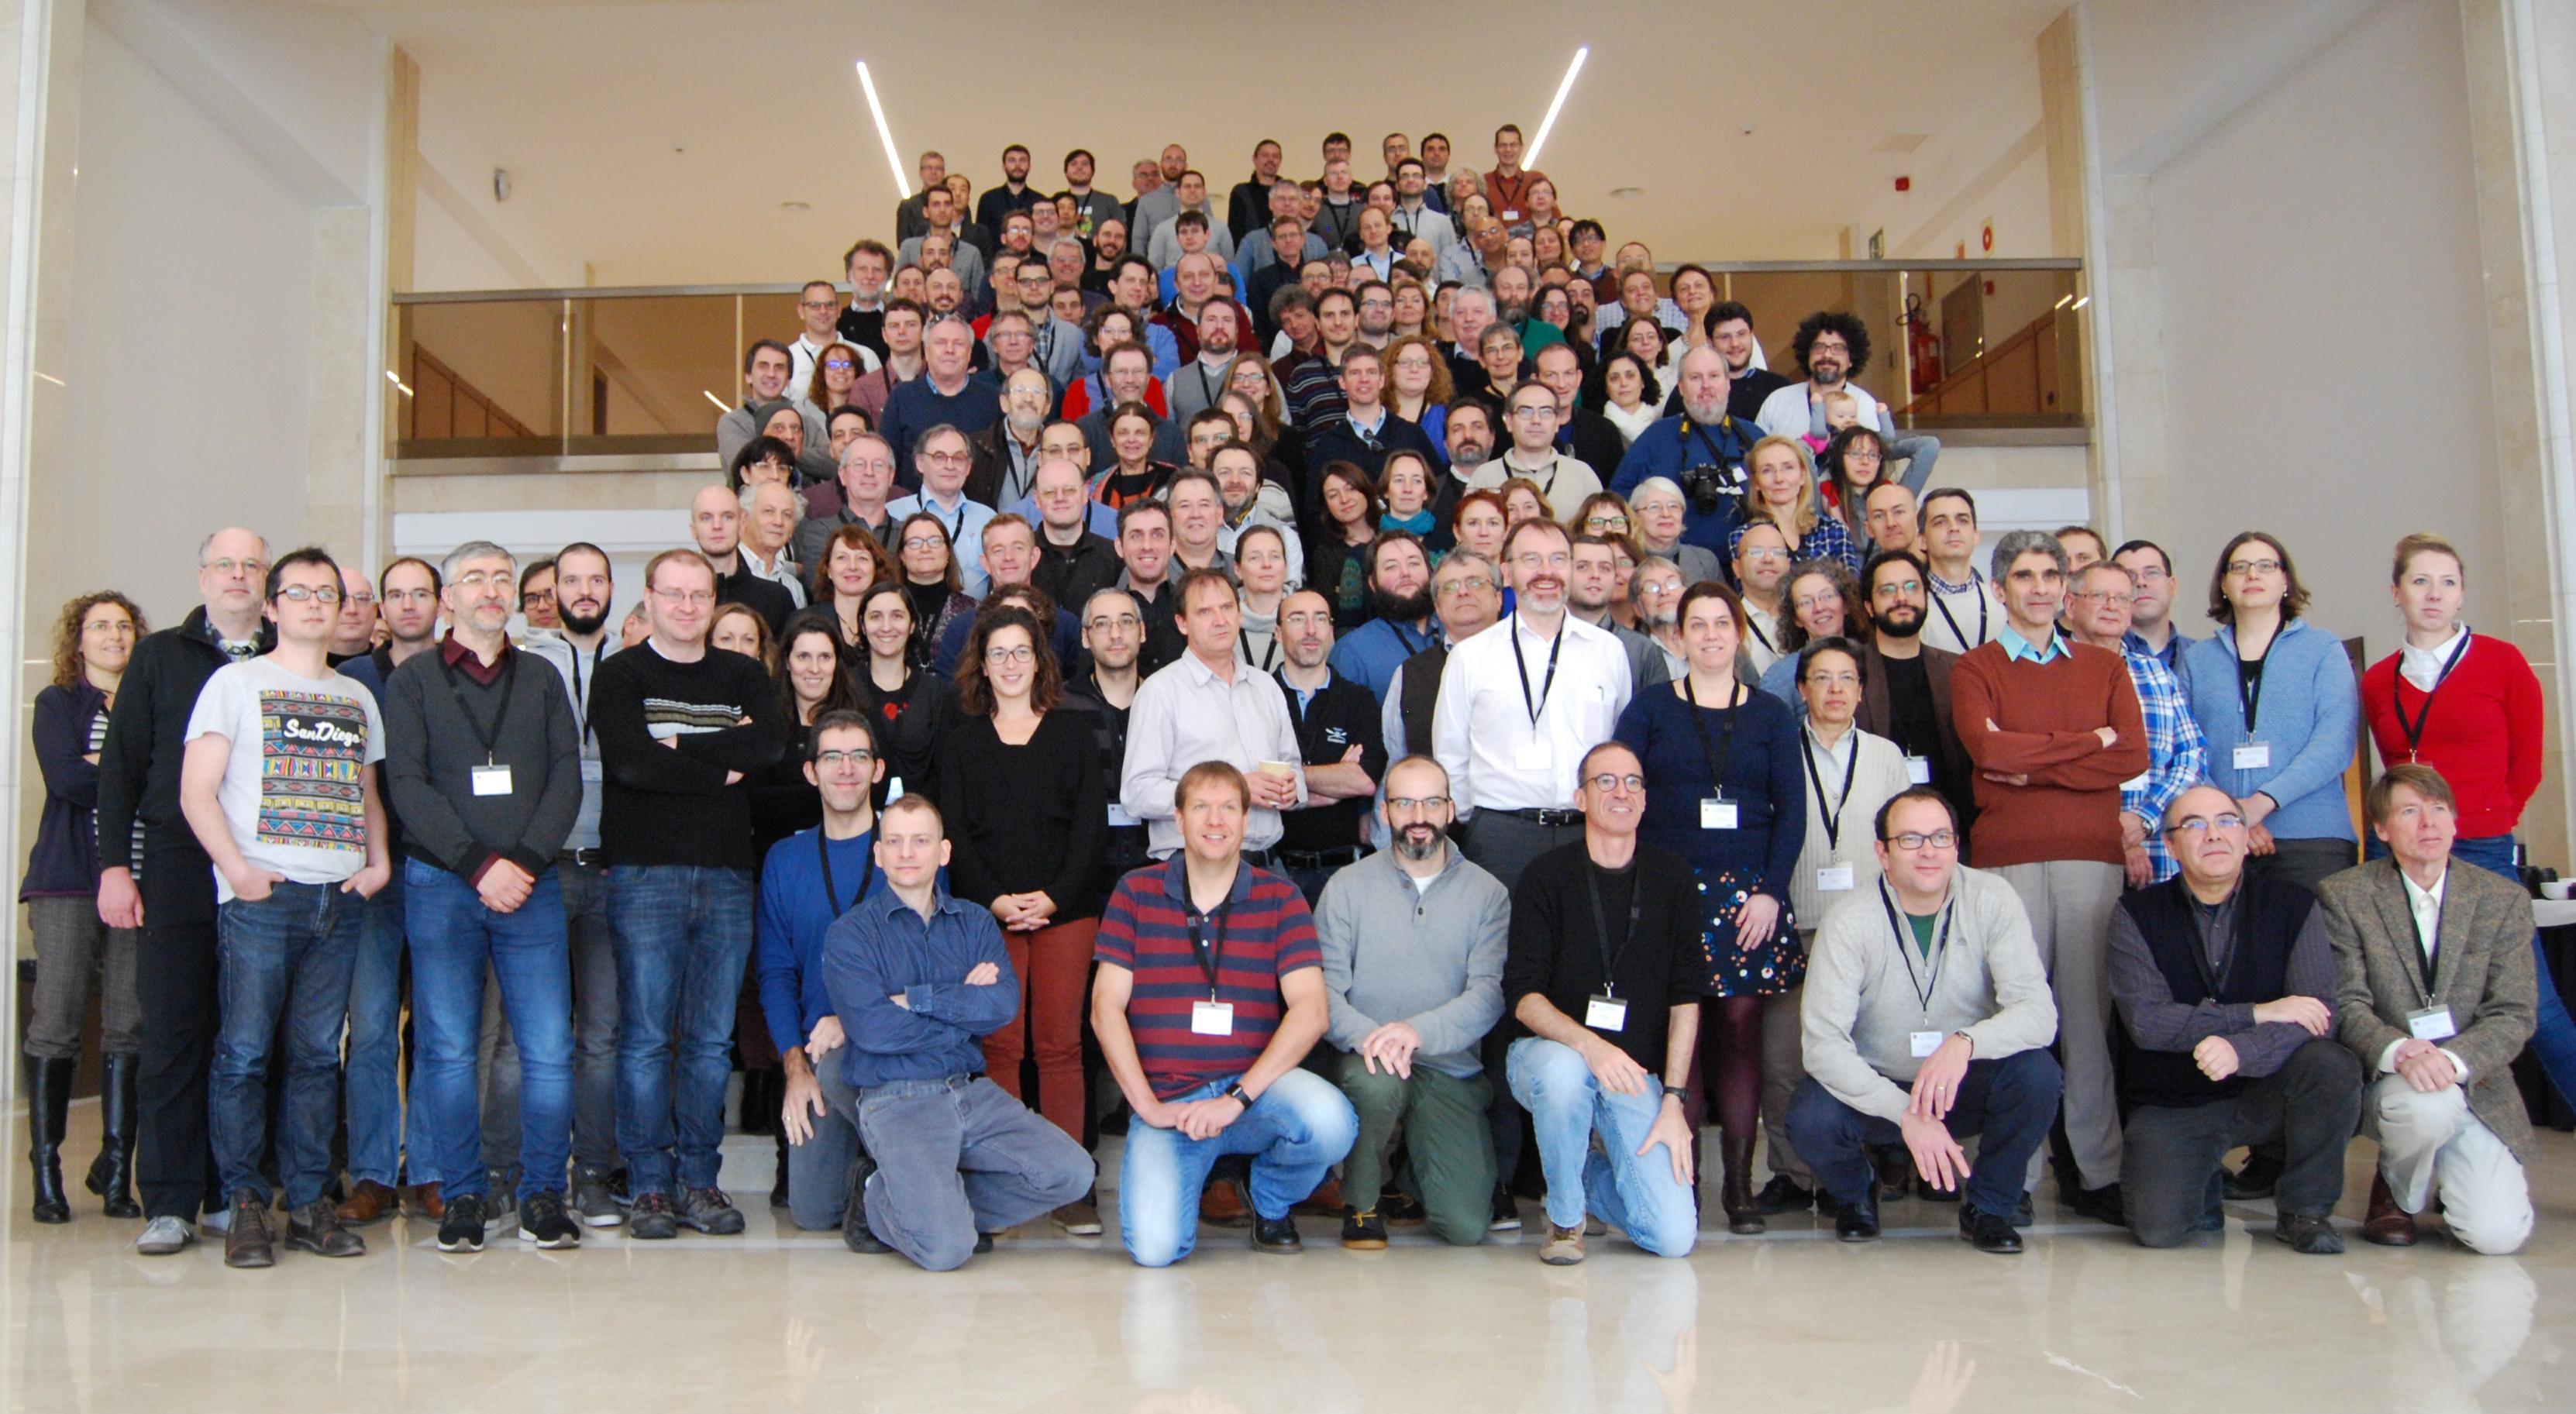
\includegraphics[width=1\linewidth]{revistas/002/imaxes/grupogaia.jpg}
    \captionof{figure}{Participants of the 2nd DPAC Consortium Meeting in Sitges, Spain. Image credit: ESA/Gaia/DPAC}
\end{center}

\paragraph{G:} Nos últimos meses a situación xeopolítica global está cambiando e
as alianzas territorias como a Unión Europea están avanzando a un maior gasto
tecnolóxico, algo que non todo o mundo comprende ou considera necesario. Que
lle dirías a alguén que dubida da importancia de custear proxectos sobre a
exploración espacial? É algo inherente ao ser humano ir en busca de respostas
sobre o Universo ou os intereses residen na utilidade que poida supoñer para os
países?

\paragraph{A:} O universo é todo e abrangue todas as escalas. O investimento en
ciencia e tecnoloxía sempre, antes ou despois, reverte no beneficio das
sociedades que, por este razoamento, son parte do universo. E isto enténdese
mellor se as sociedades teñen un mínimo nivel de cultura científica. Por
exemplo: un software para recoñecer galaxias afastadas é útil para detectar
nódulos difusos de cancro de mama; polo tanto, seguimos investigando as
galaxias, ou gastamos só en recursos médicos? A exploración espacial é
imposible sen as telecomunicacións, e estas son posibles grazas a satélites. Ou
ben, espérase que todo o mundo coñeza El Quijote ou A Gioconda pero que o
obxectivo dun Tokamak sexa producir enerxía limpa e ilimitada por fusión, coma
no interior do Sol, iso a sociedade non ten necesidade de sabelo?

Creo que abondan os exemplos da combinación de perseguir intereses de
coñecemento \textit{per se}, cos de ciencia e tecnoloxía aplicadas. Non son
intereses incompatibles, senón que son beneficiosamente complementarios.

\paragraph{G:} Que valoración farías de como está a astrofísica en España? Cres
que coa incorporación de dous españois ao cadro de persoal de astronautas da
ESA visibilizouse a importancia das misión e investigacións espaciais?

\paragraph{A:} O nivel investigador e tecnolóxico da astrofísica española é moi
alto. Dende que se sentaron as bases dos observatorios de Canarias, Calar Alto
e Sierra Nevada, xunto coa posta en marcha de institutos de investigación
asociados, que hoxe son recoñecidos mundialmente, o avance da astrofísca é
realmente imparable. Polo número e tipo de proxectos, terrestres ou espaciais,
nos que a nosa comunidade está involucrada, dentro e fóra do país, polas
publicacións, pola calidade das teses de doutramento defendidas... por moitos
indicadores, que ademais son parámetros medibles.

Por suposto, é boa nova que a ESA incorpore máis astronautas españois aos seus
equipos, e seguro que iso si contribúe a visibilizar a relevancia das misións e
investigacións espaciais. E espero que tamén contribúa a fomentar novas
vocacións científicas e tecnolóxicas.

\paragraph{G:} Dende a túa experiencia, tes algún consello que poidas compartir
cos estudantes de física e especialmente coas mozas que estén comezando?

\paragraph{A:} O mesmo consello que me deron a min varias mestras e profesores
dende a escola primaria e o instituto, logo investigadores e investigadoras
noutras etapas máis adiante: que o intenten, que non se digan a si mesmos/as
que non van poder con aquilo que queiran conseguir. Ás veces, as cousas non
saen como esperamos, por diversas razóns, así que tamén hai que ter, digamos,
plan B ou C, para continuar no noso camiño.

Pero intentando as cousas nunca quedaremos coa dúbida, ademais de que de todas
as situacións, todas, se pode obter sempre información útil para o presente e o
futuro. Ou, incluso e posiblemente, para reinterpretar o pasado.

\end{multicols}
\end{refsection}
